\documentclass[11pt]{report}
\title{Predator Prey Model}
\author{Names Here}
\date{November 2011}

\usepackage{tikz}
\usepackage{verbatim} 
\usepackage{pict2e}
\usepackage[pdftex]{hyperref}
%%%%% Remove URL link boxes %%%%%%%%%%%%%%%%%%%%%%%%%%%%%%%%%%%%%%
\hypersetup{
    colorlinks,%
    citecolor=black,%
    filecolor=black,%
    linkcolor=black,%
    urlcolor=black
}
\usepackage{times}

%%%%% Code Constraints %%%%%%%%%%%%%%%%%%%%%%%%%%%%%%%%%%%%%%%%%%%%
\usepackage{listings}
 \usepackage{courier}
%\lstset{
\lstset{columns=fullflexible,
language=Java,
%captionpos=b,
basicstyle=\footnotesize,
keywordstyle=\bfseries\ttfamily\color[rgb]{0,0,1},
identifierstyle=\ttfamily,
commentstyle=\color[rgb]{0.133,0.545,0.133},
stringstyle=\ttfamily\color[rgb]{0.627,0.126,0.941},
showstringspaces=false,
%basicstyle=\small,
numberstyle=\footnotesize,
numbers=left,
stepnumber=1,
numbersep=5pt,
tabsize=1,
breaklines=true,
%prebreak = \raisebox{0ex}[0ex][0ex]{\ensuremath{\hookleftarrow}},
breakatwhitespace=false,
aboveskip={1.5\baselineskip},
columns=fixed,
%upquote=true,
extendedchars=true,
%frame=bottomline,
inputencoding=utf8
}
%%%%%%%%%%%%%%%%%%%%%%%%%%%%%%%%%%%%%%%%%%%%%%%%%%%%%%%%%%%%%%%%%

\begin{document}

\usetikzlibrary{shapes,arrows}


\tikzstyle{block} = [rectangle, draw, fill=blue!20, 
    text width=5em, text centered, rounded corners, minimum height=4em]
\tikzstyle{line} = [draw, -latex']

\maketitle

\begin{abstract}
\end{abstract}

\tableofcontents

\chapter{Introduction}

% i just wrote this to get the report started - feel free to change or add to it

In this task we worked as a group to implement a 2D, sequential predator-prey algorithm with spatial diffusion
in Java. We tried to design the program in such a way as to take advantage of Java's object-orientated, modular nature. 
Due to the large size of our group we also decided to develop a GUI for the program, although the code was designed 
in such a way as to be usable from the command line as well. -----is it?-----\newline{}

There is always some compromise between readability and performance in coding, and we tried to keep this balance in mind
when designing our code. We made best use of class structure whilst still keeping our implementation of the given 
algorithm as efficient as possible.\newline{}

The predator prey algorithm implemented in this project crudely models the interaction between population densities of different animals, specifically Hares and Pumas. Each population has a self-interaction coefficient (birth for Hares, death for Pumas) and a coefficient describing how it interacts with other species' populations. \newline{}

These populations exist on a `world' consisting of land and water, and are also able to diffuse across land squares with a rate determined by a diffusion coefficient. Thus, each population has N+1 coefficients which determine it's behaviour, where N is the number of animals.

\chapter{Model} %dmitry

$H_{ij}^{new}=H_{ij}^{old} + {\Delta}t(C_{1}H_{ij}^{old}+C_{2}H_{ij}^{old}P_{ij}^{old} + l(H_{i+1j}^{old} + H_{i-1j}^{old} + H_{ij+1}^{old} + H_{ij-1}^{old}-H_{ij}^{old}))$


\vspace{30 mm}

\noindent for k=1:NumberOfAnimals\newline{}
if (k=ThisAnimal) then\newline{}
$N_{k}^{new}=N_{k}^{old} + {\Delta}tC_{k}(k)N_{k}^{old}$\newline{}
else\newline{}
$N_{k}^{new}=N_{k}^{old} + {\Delta}tC_{k}(k)N_{k}^{old}N_{ThisAnimal}^{old}$\newline{}
end if\newline{}
end

where

\[ C_{Hare} = \left( \begin{array}{cc}
H & PH \end{array} \right)\]    


\chapter{Design \& Implementation}
   \section{Code}
      \subsection{Structure} %simon (dmitry to make flowchart)
      %not sure if this is quite right but a first go at the code structure explanaion
          The language our group decided to code the predator-prey model in was java. Using java gave us easy access to numerous tools for creating a gui, JAVAdoc API and the main advantage for most of us was the familiarity of working with object orientated code. Object orientation provided us with the opportunity to design the central workings of the code with extensive extendibility, leaving just the user interface specifically designed for the problem at hand. The main code was split into Input, Output, GUI, Animal and Grid Algorithm classes classes which covers the different requirements of the program. A main class, PredPrey, governs the creation of occurrences of all of the other classes in the order required.  When running to program there is an option to run with or without a GUI, this is  implemented by either passing the input file names in the command line when running the program or not. If the arguments are passed, the input parameters are read from the file, if they are not then the user can input them in themselves. The parameters required by the user are the coefficients that govern the central update equation, the time step, diffusion rates of Pumas and Hares and the differential interaction coefficients between the animals, all described in ***section***.
          The input class is responsible for reading the file which holds where the land and water are. It reads the information from the file into a two dimensional array and from there calculates the number of nearest neighbours each cell has and holds that in a new two dimensional array. Water cells are held as -1 to differentiate between land cells with no neighbours and water. This array of neighbours is all that is required by the rest of the program.
          The Animal class holds it's name and all the information required about each animal and their interactions with others. Upon creation an object of the animal class is passed the number of animals in the simulation and the size of the map; initialising the arrays to hold the animals density distribution and interaction coefficients to the correct size. The values are then passed from the GUI/input file using setter methods, to set the differential coefficients, diffusion coefficients and time step for the animal. The Animal classes main function is that it holds the method which is called to update the densities in a cell on the grid. This class has been designed so that a program can be extended from this one to take any number of animals interacting to first order with each other.
          The Grid Algebra class governs methods for updating the animal densities across the  grid. The constructor takes an array of animals passed from the main class and the 2 dimensional array of neighbours passed from the input class. Upon creation the GridAlg class initialises the densities of each animal in each grid cell to a uniformly distributed random number between 0 and 1, if different density distributions were required for each animal it would be easy to edit the code to accommodate this. A couple of different methods of updating the grid are held in the class, either updating in parallel, for all animals (all of the old densities are replaced by new one's at the same time) or updating the animals one by one. Other update methods which would be interesting to investigate would be updating the cells one by one and updating random cells and or animals. In this experiment only the fully parallel update is used for investigation.
          The output class takes the density distribution of the animals every ***time steps, calculates and outputs the average density as well as an image of the density distribution. All that is passed to methods in this class from the program is the density array of an animal and a file name for saving as output. 
      \subsection{Algorithm} %matt
      \subsection{Input/Output} %milena
      
          
       
           % Here is some stuff about input and output. Not finished yet. Still needs some things to be added (or removed). Feel free to change it! 
      
      Computers cannot deal with continuous data; therefore, when modelling any kind of a system, discrete approximations must be used instead. This means that to see, for example, how a particular system evolves in time one needs to represent it by a sequence of events occurring one after another and separated by discrete time steps. 
      %The system considered in this project is a "world" or landscape consisting of land and water, the former being inhabited by a population of pumas (predators) and hares (prey).
      \newline{}
      In our model the "world", or landscape, is represented by a rectangular grid of alterable dimensions $N \times N$, where $N$ can be as large as 2000.
      We designed the code in a way such that it can read in an ASCII file that contains a set of numbers, those being either 0 or 1 and representing water and land, respectively, parses them and stores in a two-dimensional array. This means that the code can be used to model landscapes of different sizes with various distributions of land and water.
      \newline{}
      The boundary conditions are assigned to the model by setting the values for density of both, pumas and hares, to 0 at the edges of the grid.      
      \newline{}
      The initial values for the densities of pumas and hares are chosen randomly from a range of numbers between ******dMin and dMax ****** and distributed across the land cells. All these tasks are implemented in methods within the InOut class.
      The initial values for parameters that appear in the partial differential equations governing the evolution of the system with time can be set up by the user, who will be able to interact with the program by means of Graphical User Interface (GUI). Specifically, it is allowed for the user to initialise the values for the birth, death and diffusion rates of both types of animals as well as the time step ($dt$), which controls how often the system is updated with new data.  The user can also control the frequency of creating the output files, by choosing a value for the parameter $T$ in the GUI window. The output gets created every $T$ time steps. We have also included an optional "range" feature which allows the user to set a range of initial values for all the differential coefficients and an increment. In this case the code will run several times creating separate outputs for every simulation. 
      \newline{}
      Alternatively, the user can execute the code directly from within the terminal using the command line ******list of arguments or a file??*******. In the next section we talk about the GUI in more detail. 
      \newline{}
      \newline{}
      
      The methods responsible for creating the output are included in the Output class. Depending on the user's preference, the code will create one output directory (for single initial values) or a number of such directories (for the range of initial values), i.e. one for each run. In both cases the user will be able to view the distribution of both populations across the landscape every $T$ time steps. The form of the output is a number of *.ppm files which can be viewed as images, or "maps", similar to these showed in the ****FIGURE******.
      \newline{}
      % We could put one of the images here. or two maybe, one for pumas and one for hares?
      \newline{}
      The number of the *.ppm files created depends on the initial parameters specified by the user, $dt$ and $T$. To maximise the level of output clarity we decided to make separate landscape "maps" for each type of animal, here pumas and hares. In each "map" the pixels corresponding to water cells are shown in blue, while the land cells are white. The variation in density of pumas/hares across the land cells is represented by different shades of grey, with black colour corresponding to the maximum value. 
      \newline{}
      For each type of animal, every $T$ time steps, the code also calculates the mean population density and writes it along with the corresponding time into a file. 
      

      
      	
      
      
      \subsection{GUI} %dmitry
   
   \section{Tools}
      \subsection{SVN} %matt
      \subsection{Makefile} %tom
      \subsection{Unit Testing} %jorge
      Every class of the project form a functional unit according to the design elaborated at the beginning of the \newline{}
  has been tested using the Java JUnit framework \newline{}
The libraries necessary to the tests are thus accessed from the test cases using Java import statements and extending the TestCase superclass in the class declaration:

\begin{lstlisting}[language=Java,caption= Test case headers]
import org.junit.Before;
import org.junit.Test;
import junit.framework.TestCase;

public class TestAnimal extends TestCase {
...
\end{lstlisting}

Then the test cases, for each class, follow the normal directives in use for Unit testing with JUnit. The most relevant methods were submitted to thorough tests, where their properties, return values and correct functioning were evaluated by comparing the actual results they provide with the expected ones. These procedures were implemented by test methods in each test case using the format required by the JUnit standards. 

Every test case included a setup() method that builds the initial object and its different parameters. Directives like @Before and @Test for every method declaration were thus inserted in the code were appropriate. The functioning of a method is then assessed comparing the expected results with the actual ones with JUnit testing methods such as AssertEquals(), AssertNotNull(), etc.

\begin{lstlisting}[language=Java,caption= Use of JUnit directives in test cases]
@Before
public void setUp() {
    ...
    testAnimal = new Animal(numbAnimals);
    testAnimal.setName("Puma");
    testAnimal.setDiffCo(diffCoIn);
    ...
@Test
public void testAnimal() {
    assertNotNull(testAnimal);
    assertNotNull(testAnimal2);
} 
...
\end{lstlisting}

\chapter{Performance Analysis}
   \section{Testing} %chen+tom
   
   Tests were preformed in order to profile the code's performance and scalability. The unix \emph{time} command was 
   used to time the code runs, with `user' and `system' time being summed to find the total computation time.\newline{}
   
   The relationship between total computation time per cell and the number of cells was measured in order to quantify the overhead
   needed by the code (see Figure \ref{overhead}). We found that, below a grid size of $\sim$100 by 100, overhead became important, whereas at 
   larger grid sizes the computation time scaled linearly with the total number of cells. Any scaling worse than linear (such as 
   total computation time being proportional to the NumberOfCells$^{1.2}$ would be a huge (and unnecessary) inefficiency, especially with larger grids.\newline{}
   
   Some overhead is inevitable in any code, but the amount of effort put into simplifying a problem (such as creating arrays of neighbours)
   should depend on the expected size of the problem. Our code could probably have had less overhead, allowing it to run faster with smaller grid sizes,
   but this would likely led to it having a worse (linear) scaling with cell number.
   
   
   
   \section{Analysis} %tom+chen
   
   \begin{figure}[h]
   
   % GNUPLOT: LaTeX picture with Postscript
\begingroup
  \makeatletter
  \providecommand\color[2][]{%
    \GenericError{(gnuplot) \space\space\space\@spaces}{%
      Package color not loaded in conjunction with
      terminal option `colourtext'%
    }{See the gnuplot documentation for explanation.%
    }{Either use 'blacktext' in gnuplot or load the package
      color.sty in LaTeX.}%
    \renewcommand\color[2][]{}%
  }%
  \providecommand\includegraphics[2][]{%
    \GenericError{(gnuplot) \space\space\space\@spaces}{%
      Package graphicx or graphics not loaded%
    }{See the gnuplot documentation for explanation.%
    }{The gnuplot epslatex terminal needs graphicx.sty or graphics.sty.}%
    \renewcommand\includegraphics[2][]{}%
  }%
  \providecommand\rotatebox[2]{#2}%
  \@ifundefined{ifGPcolor}{%
    \newif\ifGPcolor
    \GPcolortrue
  }{}%
  \@ifundefined{ifGPblacktext}{%
    \newif\ifGPblacktext
    \GPblacktexttrue
  }{}%
  % define a \g@addto@macro without @ in the name:
  \let\gplgaddtomacro\g@addto@macro
  % define empty templates for all commands taking text:
  \gdef\gplbacktext{}%
  \gdef\gplfronttext{}%
  \makeatother
  \ifGPblacktext
    % no textcolor at all
    \def\colorrgb#1{}%
    \def\colorgray#1{}%
  \else
    % gray or color?
    \ifGPcolor
      \def\colorrgb#1{\color[rgb]{#1}}%
      \def\colorgray#1{\color[gray]{#1}}%
      \expandafter\def\csname LTw\endcsname{\color{white}}%
      \expandafter\def\csname LTb\endcsname{\color{black}}%
      \expandafter\def\csname LTa\endcsname{\color{black}}%
      \expandafter\def\csname LT0\endcsname{\color[rgb]{1,0,0}}%
      \expandafter\def\csname LT1\endcsname{\color[rgb]{0,1,0}}%
      \expandafter\def\csname LT2\endcsname{\color[rgb]{0,0,1}}%
      \expandafter\def\csname LT3\endcsname{\color[rgb]{1,0,1}}%
      \expandafter\def\csname LT4\endcsname{\color[rgb]{0,1,1}}%
      \expandafter\def\csname LT5\endcsname{\color[rgb]{1,1,0}}%
      \expandafter\def\csname LT6\endcsname{\color[rgb]{0,0,0}}%
      \expandafter\def\csname LT7\endcsname{\color[rgb]{1,0.3,0}}%
      \expandafter\def\csname LT8\endcsname{\color[rgb]{0.5,0.5,0.5}}%
    \else
      % gray
      \def\colorrgb#1{\color{black}}%
      \def\colorgray#1{\color[gray]{#1}}%
      \expandafter\def\csname LTw\endcsname{\color{white}}%
      \expandafter\def\csname LTb\endcsname{\color{black}}%
      \expandafter\def\csname LTa\endcsname{\color{black}}%
      \expandafter\def\csname LT0\endcsname{\color{black}}%
      \expandafter\def\csname LT1\endcsname{\color{black}}%
      \expandafter\def\csname LT2\endcsname{\color{black}}%
      \expandafter\def\csname LT3\endcsname{\color{black}}%
      \expandafter\def\csname LT4\endcsname{\color{black}}%
      \expandafter\def\csname LT5\endcsname{\color{black}}%
      \expandafter\def\csname LT6\endcsname{\color{black}}%
      \expandafter\def\csname LT7\endcsname{\color{black}}%
      \expandafter\def\csname LT8\endcsname{\color{black}}%
    \fi
  \fi
  \setlength{\unitlength}{0.0500bp}%
  \begin{picture}(7200.00,4536.00)%
    \gplgaddtomacro\gplbacktext{%
      \csname LTb\endcsname%
      \put(1100,640){\makebox(0,0)[r]{\strut{}-3.5}}%
      \put(1100,1111){\makebox(0,0)[r]{\strut{}-3.0}}%
      \put(1100,1582){\makebox(0,0)[r]{\strut{}-2.5}}%
      \put(1100,2053){\makebox(0,0)[r]{\strut{}-2.0}}%
      \put(1100,2523){\makebox(0,0)[r]{\strut{}-1.5}}%
      \put(1100,2994){\makebox(0,0)[r]{\strut{}-1.0}}%
      \put(1100,3465){\makebox(0,0)[r]{\strut{}-0.5}}%
      \put(1100,3936){\makebox(0,0)[r]{\strut{} 0.0}}%
      \put(1220,440){\makebox(0,0){\strut{} 0}}%
      \put(2167,440){\makebox(0,0){\strut{} 1}}%
      \put(3113,440){\makebox(0,0){\strut{} 2}}%
      \put(4060,440){\makebox(0,0){\strut{} 3}}%
      \put(5007,440){\makebox(0,0){\strut{} 4}}%
      \put(5953,440){\makebox(0,0){\strut{} 5}}%
      \put(6900,440){\makebox(0,0){\strut{} 6}}%
      \put(400,2288){\rotatebox{90}{\makebox(0,0){\strut{}log$_{10}$ Time/Cell [s]}}}%
      \put(4060,140){\makebox(0,0){\strut{}log$_{10}$ Number of Cells}}%
      \put(4060,4236){\makebox(0,0){\strut{}Run Time/Number of Cells vs. Number of Cells}}%
    }%
    \gplgaddtomacro\gplfronttext{%
      \csname LTb\endcsname%
      \put(5997,3773){\makebox(0,0)[r]{\strut{}Run Time/Number of Cells}}%
    }%
    \gplbacktext
    \put(0,0){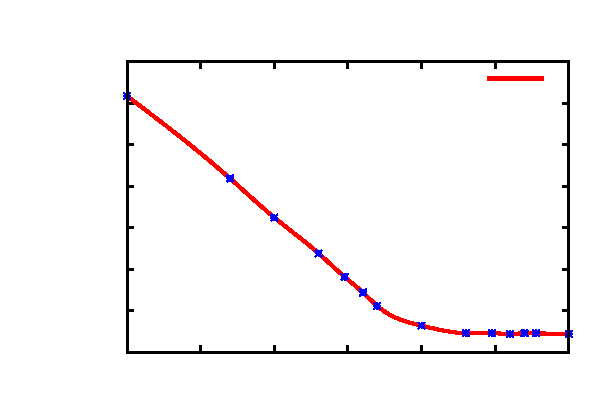
\includegraphics{figs/overhead}}%
    \gplfronttext
  \end{picture}%
\endgroup

   \caption{\label{overhead}This is a graph of total time spent on each cell, which shows that overheads such as array initialisation
   and output (i.e. things not directly involved in the simulation) take up a significant fraction of computation
   time with grids smaller than $\sim$100 by 100.}
   \end{figure}

  




\chapter{Conclusions} %everyone

   \begin{figure}[h]
   
   % GNUPLOT: LaTeX picture with Postscript
\begingroup
  \makeatletter
  \providecommand\color[2][]{%
    \GenericError{(gnuplot) \space\space\space\@spaces}{%
      Package color not loaded in conjunction with
      terminal option `colourtext'%
    }{See the gnuplot documentation for explanation.%
    }{Either use 'blacktext' in gnuplot or load the package
      color.sty in LaTeX.}%
    \renewcommand\color[2][]{}%
  }%
  \providecommand\includegraphics[2][]{%
    \GenericError{(gnuplot) \space\space\space\@spaces}{%
      Package graphicx or graphics not loaded%
    }{See the gnuplot documentation for explanation.%
    }{The gnuplot epslatex terminal needs graphicx.sty or graphics.sty.}%
    \renewcommand\includegraphics[2][]{}%
  }%
  \providecommand\rotatebox[2]{#2}%
  \@ifundefined{ifGPcolor}{%
    \newif\ifGPcolor
    \GPcolortrue
  }{}%
  \@ifundefined{ifGPblacktext}{%
    \newif\ifGPblacktext
    \GPblacktexttrue
  }{}%
  % define a \g@addto@macro without @ in the name:
  \let\gplgaddtomacro\g@addto@macro
  % define empty templates for all commands taking text:
  \gdef\gplbacktext{}%
  \gdef\gplfronttext{}%
  \makeatother
  \ifGPblacktext
    % no textcolor at all
    \def\colorrgb#1{}%
    \def\colorgray#1{}%
  \else
    % gray or color?
    \ifGPcolor
      \def\colorrgb#1{\color[rgb]{#1}}%
      \def\colorgray#1{\color[gray]{#1}}%
      \expandafter\def\csname LTw\endcsname{\color{white}}%
      \expandafter\def\csname LTb\endcsname{\color{black}}%
      \expandafter\def\csname LTa\endcsname{\color{black}}%
      \expandafter\def\csname LT0\endcsname{\color[rgb]{1,0,0}}%
      \expandafter\def\csname LT1\endcsname{\color[rgb]{0,1,0}}%
      \expandafter\def\csname LT2\endcsname{\color[rgb]{0,0,1}}%
      \expandafter\def\csname LT3\endcsname{\color[rgb]{1,0,1}}%
      \expandafter\def\csname LT4\endcsname{\color[rgb]{0,1,1}}%
      \expandafter\def\csname LT5\endcsname{\color[rgb]{1,1,0}}%
      \expandafter\def\csname LT6\endcsname{\color[rgb]{0,0,0}}%
      \expandafter\def\csname LT7\endcsname{\color[rgb]{1,0.3,0}}%
      \expandafter\def\csname LT8\endcsname{\color[rgb]{0.5,0.5,0.5}}%
    \else
      % gray
      \def\colorrgb#1{\color{black}}%
      \def\colorgray#1{\color[gray]{#1}}%
      \expandafter\def\csname LTw\endcsname{\color{white}}%
      \expandafter\def\csname LTb\endcsname{\color{black}}%
      \expandafter\def\csname LTa\endcsname{\color{black}}%
      \expandafter\def\csname LT0\endcsname{\color{black}}%
      \expandafter\def\csname LT1\endcsname{\color{black}}%
      \expandafter\def\csname LT2\endcsname{\color{black}}%
      \expandafter\def\csname LT3\endcsname{\color{black}}%
      \expandafter\def\csname LT4\endcsname{\color{black}}%
      \expandafter\def\csname LT5\endcsname{\color{black}}%
      \expandafter\def\csname LT6\endcsname{\color{black}}%
      \expandafter\def\csname LT7\endcsname{\color{black}}%
      \expandafter\def\csname LT8\endcsname{\color{black}}%
    \fi
  \fi
  \setlength{\unitlength}{0.0500bp}%
  \begin{picture}(7200.00,5040.00)%
    \gplgaddtomacro\gplbacktext{%
      \csname LTb\endcsname%
      \put(860,640){\makebox(0,0)[r]{\strut{} 0}}%
      \put(860,1400){\makebox(0,0)[r]{\strut{} 1}}%
      \put(860,2160){\makebox(0,0)[r]{\strut{} 2}}%
      \put(860,2920){\makebox(0,0)[r]{\strut{} 3}}%
      \put(860,3680){\makebox(0,0)[r]{\strut{} 4}}%
      \put(860,4440){\makebox(0,0)[r]{\strut{} 5}}%
      \put(980,440){\makebox(0,0){\strut{} 0}}%
      \put(2164,440){\makebox(0,0){\strut{} 100}}%
      \put(3348,440){\makebox(0,0){\strut{} 200}}%
      \put(4532,440){\makebox(0,0){\strut{} 300}}%
      \put(5716,440){\makebox(0,0){\strut{} 400}}%
      \put(6900,440){\makebox(0,0){\strut{} 500}}%
      \put(400,2540){\rotatebox{90}{\makebox(0,0){\strut{}Density}}}%
      \put(3940,140){\makebox(0,0){\strut{}Time [s]}}%
      \put(3940,4740){\makebox(0,0){\strut{}Population Density vs. Time}}%
    }%
    \gplgaddtomacro\gplfronttext{%
      \csname LTb\endcsname%
      \put(5997,4277){\makebox(0,0)[r]{\strut{}Hares}}%
      \csname LTb\endcsname%
      \put(5997,4077){\makebox(0,0)[r]{\strut{}Pumas}}%
    }%
    \gplbacktext
    \put(0,0){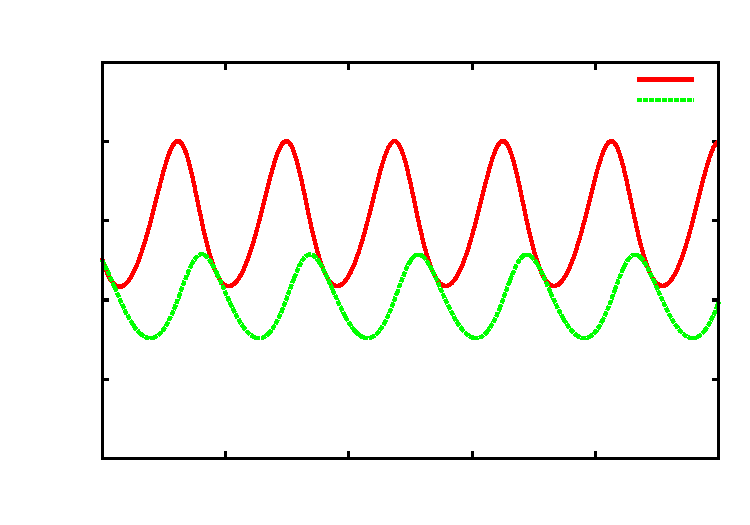
\includegraphics{figs/density}}%
    \gplfronttext
  \end{picture}%
\endgroup

   \caption{Population density vs. time for Hares and Pumas. This periodic behaviour is typical of predator-prey interactions.}
   \end{figure}

\chapter{Group Evaluation} %everyone

\end{document}
